\begin{figure}[t]
  \centering
  \begin{subfigure}[b]{0.4\textwidth}
    \centering
    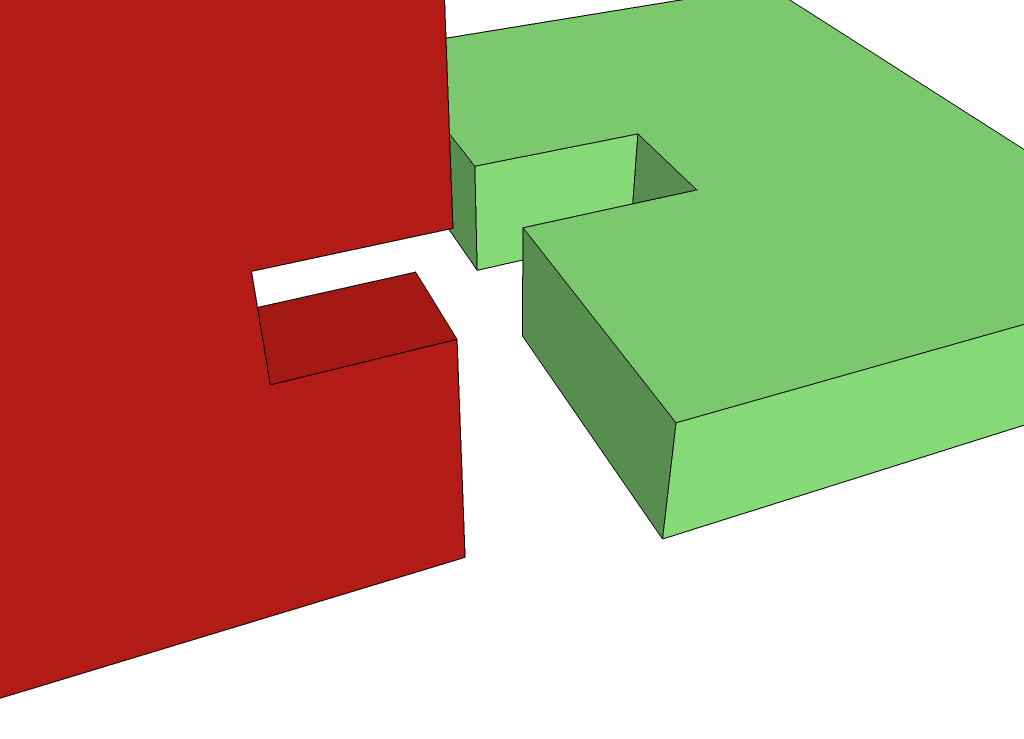
\includegraphics[width=\textwidth]{img/joint-notch.png}
    \caption{Notch joints.}
    \label{fig:joint-notch}
  \end{subfigure}
  \hspace{8mm}
  \begin{subfigure}[b]{0.4\textwidth}
    \centering
    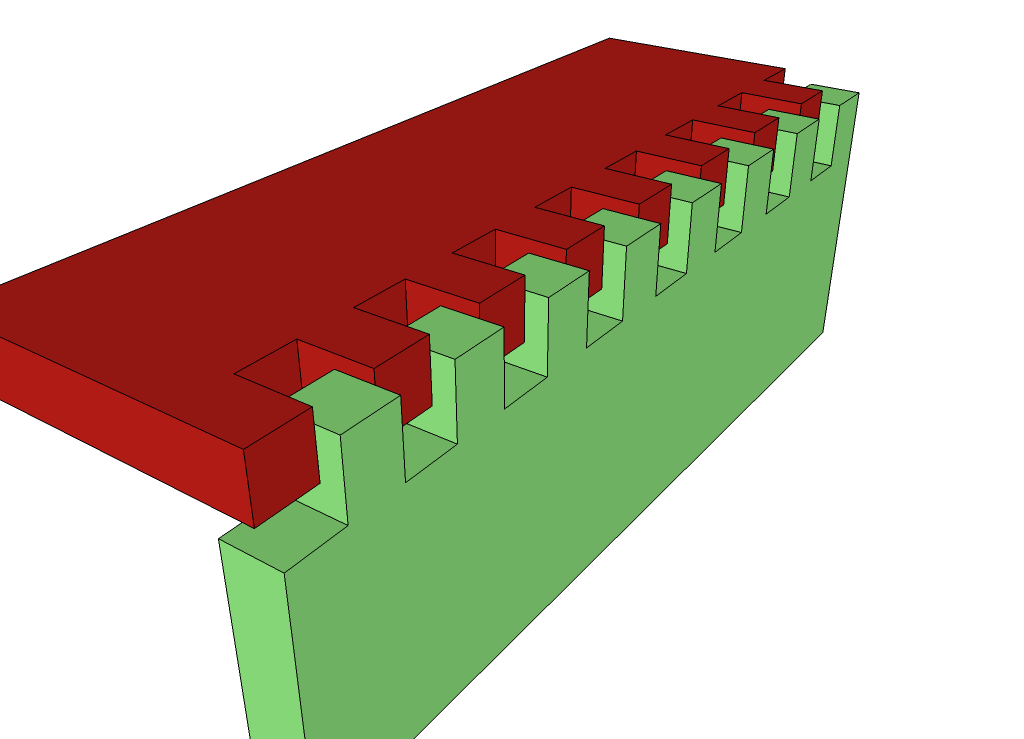
\includegraphics[width=\textwidth]{img/joint-finger.png}
    \caption{Finger (box) joints.}
    \label{fig:joint-finger}
  \end{subfigure}
  \caption[Two Common Notch Types]{Two common methods to join
      parts. Notch joints are used when parts intersect along part
      midsections; finger joints (box joints) join parts along edges.}
  \label{fig:joint}
\end{figure}
